% !TeX spellcheck = cs_CZ
{\tikzset{external/prefix={tikz/MAI/}}
 \tikzset{external/figure name/.add={ch05_}{}}
%---------------------------------------------------------------------------------------------------
% file: Differential_Calculus_applications.tex
%---------------------------------------------------------------------------------------------------
\chapter{Aplikace diferenciálního počtu}\label{chap:Apl_dif_poc}
\minitoc

%================Kapitola: Aplikace diferenciálního počtu =========================================
Diferenciální počet má rozsáhlou oblast užití. V této kapitole ukážeme použití výsledků předchozích 
kapitol k vyšetřování průběhu funkce a vlastnosti rovinných křivek. 
  \section{Průběh funkce}
    Pomocí derivace můžeme studovat vlastnosti funkce, které usnadní vyšetřování jejího průběhu.  
    \subsection{Monotonie funkcí}
      Jednou z důležitých vlastností funkce je její \textquotedblleft monotonie\textquotedblright, 
      kterou jsme definovali již v odst. \ref{MA1:subsec_vlastnosti_funkce} kap. 
      \ref{mai:IchapIII}. Proto je při vyšetřování průběhu funkce důležité určit množiny (často 
      jsou to intervaly), na nichž je funkce monotónní, jinak řečeno, najít \textquotedblleft 
      intervaly monotonie funkce\textquotedblright (viz \cite[s.~208]{Brabec1989}). 
    \begin{enumerate}
      \item Zjistíme \textbf{definiční obor funkce}, vyjádříme jej v intervalech a z nich poznáme,  
            kde je funkce \textbf{spojitá}. Funkce je spojitá v $(a,b)$ pro každý bod tohoto 
            intervalu, když$|f(x)-f(c)|<\varepsilon$, kde $\varepsilon>0$ je libovolně zvolené 
            číslo, a pro všechna $x$ z okolí bodu $c$ je $|x-c|<\delta$, kde $\delta>0$ je na 
            $\varepsilon$ nezávislé.
      \item Určíme, je-li funkce \textbf{lichá} $f(-x)=-f(x)$ nebo \textbf{sudá} $f(-x)=f(x)$.   
            Je-li funkce lichá, je souměrná podle středu souměrnosti (obyčejně to bývá počátek 
            souřadnic $xy$), je-li sudá, je souměrná podle osy $y$.
      \item Určíme \emph{průsečíky křivky s osami pravoúhlých souřadnic}. Body, ve kte\-rých 
            křivka  protíná osu $x$ spolu s body, ve kte\-rých není křivka spojitá, rozlišují 
            intervaly, v nichž je graf křivky nad osou $x$ od intervalů, ve kterých je graf křivky 
            pod osou $x$.
      \item V krajních bodech definičních intervalů, ve kterých je funkce spojitá, stano\-víme 
      \emph{limity funkce} a dále $$\lim_{x \to \pm \infty}f(x).$$
      \item Vypočítáme $f'(x)$ a $f''(x)$, abychom zjistily, kde je funkce \emph{rostoucí}     
            $f'(x)>0$, \emph{klesající} $f'(x)<0$ a kde jsou \emph{lokální extrémy}. Dostaneme-li 
            dosazením kořenů rovnice $f'(x)=0$ do $f''(x)$ hodnotu $f''(x)>0$, má funkce lokální 
            minimum, při $f''(x)<0$ má funkce lokální maximum. V intervalech, kde $f''(x)>0$, je 
            křivka \textbf{konvexní (vypuklá)}, kde $f''(x)<0$, je křivka \textbf{konkávní 
            (vydutá)}. Body, v nichž $f''(x)$ mění znaménko, jsou \textbf{inflexní body}. Najdeme 
            je tak, že stanovíme hodnoty $x$, pro které je $f''(x)=0$ nebo neexistuje. Číslo $c$ je 
            inflexní bod, když existuje takové okolí bodu $c$, že pro $x>c$ je oblouk křivky 
            konvexní a pro $x<c$ konkávní. Je nutné si uvědomit, že když má $f'(x)$ konečnou 
            derivaci, je inflexní bod $c$ taky nulovým bodem druhé derivace čili kořenem rovnice 
            $f''(x)=0$. Obrácená věta neplatí, tj. z $f''(x)=0$ nevyplývá, že v bodě $c$ má $f'(x)$ 
            extrém a že bod $c$ je inflexním bodem.
      \item \textbf{Asymptota} je tečna křivky $f(x)$, jejíž bod dotyku je v nekonečnu. Platí-li  
            $$\lim_{x \to a}f(x) =  \pm\infty,$$ je přímka $x=a$ její asymptotou. Jinak asymptoty 
            mají rovnici $y=kx+q$, kde $x$ a $y$ jsou souřadnice bodů na asymptotách. Existují-li 
            konečné limity $$\lim_{x \to \pm\infty}\frac{f(x)}{x}=k$$  a $$\lim_{x \to 
            \pm\infty}[f(x)-kx] =q$$ pak je asymptotou přímka $y=kx+q$. Můžeme-li rovnici křivky 
            rozložit (tj. rozložit její pravou stranu, oby\-čejně dělením čitatele jmenovatelem, 
            má-li tvar zlomku) na dvě části, z nichž jedna má tvar $kx+q$ a druhá zbytek 
            $\varphi(x)$, tj. $f(x)=kx+q+\varphi(x)$ a $\varphi(x)_{x\rightarrow 
            \pm\infty}\rightarrow 0$, je přímka $y=kx+q$ asymptotou.
      \item Zpřesnění grafu křivky provedeme sestavením tabulky souřadnic dalších bodů křivky,  
            tj. ke zvoleným hodnotám $x$ (z definičního oboru funkce) vypočítáme hodnoty $y$. Do 
            dalších řádků tabulky zapíšeme hodnoty  $f'(x)$ a $f''(x)$, ve kterých intervalech je 
            funkce \emph{rostoucí}, ve kterých \emph{klesá}, kde je \emph{vypuklá}, kde je 
            \emph{dutá}, kde jsou \emph{lokální extrémy}, \emph{inflexní body} apod., 
            případně sestavíme dílčí tabulky pro jednotlivé \emph{charakteristické vlastnosti} vyšetřované funkce.
    \end{enumerate}
    %-------------------- EXAM001 --------------------------------------
    % !TeX spellcheck = cs_CZ
\begin{example}\label{mai:exam003}
  Vyšetřete průběh funkce $$f(x):y=\frac{1+x^2}{1-x^2}$$
  \begin{enumerate}
    \item Definiční obor $D_f=\realset-\{±1\}=(-\infty,-1)\cup(-1,1)\cup(1,+\infty)$
    \item Funkce je sudá $$f(-x)=f(x): \frac{1+x^2}{1-x^2}=\frac{1+(-x)^2}{1-(-x)^2}.$$ Funkce  
         není periodická.
    \item Stanovíme funkční hodnoty v krajních bodech definičního obor $1, -1$ a v nevlastních  
         bodech $-\infty,+\infty$.Protože je funkce \textbf{sudá}, omezíme se jen na vyšetřování 
         nezáporné části. Nejprve vlastnosti fun\-kce v okolí bodu $1$. Ten nepatří do $D_f$ a 
         proto určíme limity funkce v pravém a levém okolí tohoto bodu. $$\lim_{x\to 
         1_{-}}=\frac{1+x^2}{1-x^2}.$$ Pro výpočet limity použijeme substituci $y=1-x^2$: 
         $$\lim_{y\to0+}\frac{2-y}{y}=+\infty$$ 
         \footnote{$\lim_{x\to0_+}\frac{1}{x}=\infty$} proto 
         $$\lim_{x\to1_{-}}\frac{1+x^2}{1-x^2}=+\infty.$$ 
         Obdobně dojdeme k $$\lim_{x\to1_+}\frac{1+x^2}{1-x^2}=-\infty.$$ A konečně v nevlastních 
         bodech $±\infty$ je limita $$\lim_{x\to±\infty}\frac{1+x^2}{1-x^2} = 
         \lim_{x\to\pm\infty}\frac{1}{1-x^2} + \lim_{x\to\pm\infty}\frac{x^2}{1-x^2}=0-1=-1.$$ 
         Výpočtem limit jsme zároveň určili dva absolutní (globální) extrémy a jeden lokální:
         \begin{itemize}
           \item v intervalu $(-1,1)$ má funkce maximum $\infty$ a minimum $1$,
           \item v intervalech $(-1,1)\cup(1,+\infty)$ má funkce minimum $-\infty$ a maximum $-1$.
         \end{itemize}
    \item Nyní vyšetříme zda, případně kolik a jaké, má funkce $f(x)$ průsečíky s osami souřadnic.  
         S osou $x$ nemá funkce žádné průsečíky, protože pro $y=0$ není definována 
         $H_f=\realset-\{-1,1\rangle$. Pro $x=0$ je $y=\frac{1+0^2}{1-0^2}=1$, proto má $f(x)$ 
         právě jeden průsečík s osou $y$ a to $[0,1]$.
    \item Zatím jsme zjistili, že naše funkce není definována v bodech $1$ a $-1$ a proto není  
         spojitá v  $\realset$. Nevíme však, jaký je její průběh v jednotlivých intervalech 
         definičního oboru.  Abychom získali názornější představu o průběhu funkce, zjistíme má-li 
         derivaci.
         \begin{align*}
           y' &= \frac{(1+x^2)'(1-x^2 )-(1+x^2)(1-x^2 )'}{(1-x^2)^2} \\
           y' &= \frac{2x(1-x^2 )-(1+x^2 )(-2x)}{(1-x^2 )^2}         \\
           y' &= \frac{4x}{(1-x^2 )^2}
         \end{align*}
         Protože má vlastní derivaci\footnote{$f(x)$ je spojitá v intervalech $(-\infty,-1), 
         (-1,1),(1,\infty)$  věta s spojité funkci}, můžeme určit její vlastnosti v intervalech 
         $\langle0,1)$ a $(1,\infty)$. V těchto intervalech je $y'>0$ a proto jde o funkci ryze 
         monotónní, rostoucí \footnote{Plyne z věty o postačujících podmínkách ryzí monotónnosti 
         funkce na intervalu} v daných intervalech \footnote{V intervalech $(-\infty,-1) 
         ,(-1,0\rangle$ je funkce klesající.}. Výpočtem zjistíme druhou derivaci funkce. 
         Ta nám pomůže určit další extrém v intervalu $\langle0,1)$ a zároveň vyšetřit 
         \textbf{konkávnost} a \textbf{konvexnost}.
         \begin{align*}
           y'' &= \frac{(4x)' (1-x^2 )^2-(4x)(1-2x^2+x^4 )'}{(1-x^2 )^4}  \\
           y'' &= \frac{4(1-2x^2+x^4 )-4x(-4x+4x^3 )}{(1-x^2 )^4}         \\
           y'' &= \frac{4(1-x^2 )(3x^2+1)}{(1-x^2 )^4}                    \\
           y'' &= \frac{4(3x^2+1)}{(1-x^2 )^3}
         \end{align*}
         Abychom mohli určit lokální extrém funkce $f(x)$ v intervalu $\langle0,1)$, pomocí druhé 
         derivace, musíme najít kořeny rovnice $f' (x)=0$. V našem případě $$y'=\frac{4x}{(1-x^2 
         )^2}\Rightarrow\frac{4x}{(1-x^2)^2}=0\rightarrow x_0=0,$$ tento kořen 
         \footnote{stacionární bod}  pak dosadíme do druhé derivace, tj. 
         $$y''(0)=\frac{4(3\cdot0^2+1)}{(1-0^2 )^3}=4,$$ protože je $f''(x)>0$, má v bodě $x_0$ 
         lokální minimum. Můžeme rovněž konstatovat, že funkce nemá inflexní body \footnote{Pro 
         existenci inflexního bodu je nutné splnění jedné z podmínek a to buď $f''(x_0)=0$, nebo 
         $f''(x_0)$ neexistuje.}. Konkávnost a konvexnost funkce v intervalech $\langle0,1)$ a 
         $(1,\infty)$ vyšetříme pomocí vlastností druhé derivace funkce. Tedy
         \begin{itemize}
           \item $\langle0,1): y''=\frac{4(3x^2+1)}{(1-x^2 )^3} >0 \Rightarrow$ funkce je v 
                 tomto intervalu \textbf{konvexní},
           \item $(1,\infty): y''=\frac{4(3x^2+1)}{(1-x^2 )^3} <0 \Rightarrow$ funkce je v tomto  
                 intervalu \textbf{konkáv\-ní}.
         \end{itemize}
    \item Z předchozích výpočtů plyne, že křivka má asymptoty $y=-1,x=\pm1$.
  \end{enumerate}
   {\centering
    \captionsetup{type=figure}
    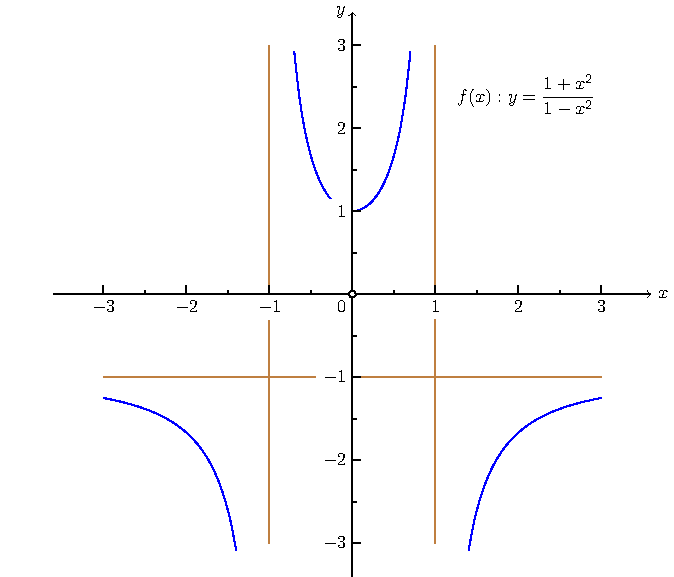
\includegraphics[width=1\linewidth]{MAI007.pdf}
    \captionof{figure}{Graf funkce $f(x):y=\dfrac{1+x^2}{1-x^2}$}
    \label{MAI:fig_007}
  \par}
\end{example}
    %-------------------------------------------------------------------

} %tikzset
%---------------------------------------------------------------------------------------------------
\printbibliography[heading=subbibliography]
\addcontentsline{toc}{section}{Seznam literatury} 